%The \introduction command is provided as a convenience.
%if you want special chapter formatting, you'll probably want to avoid using it altogether
		
\chapter*{Introduction}
    \addcontentsline{toc}{chapter}{Introduction}
		\chaptermark{Introduction}
		\markboth{Introduction}{Introduction}
% The three lines above are to make sure that the headers are right, that the intro gets included in the table of contents, and that it doesn't get numbered 1 so that chapter one is 1.

Quantum is crazy. There is nothing like it. Particle-wave duality has incredible implications, documented by experiment.

	(Important: Particle-wave association on a fluid interface (Protiere 2006)).
	    
	    In 2005, Yves Couder showed that bouncing oil drops on vertically vibrating fluid bath exhibited properties analogous to the paradoxical properties seen only at the quantum scale (CITE: Dynamical phenomena:  Walking and orbiting droplets?). Couder, John Bush, and others have shown that this system can reproduce double-slit single-particle interference, orbiting, tunneling, quantized orbits, spin, and more.
	    
	    \subsection{Quantum Motivation}
	    
	    \subsection{Bouncing Droplets}
	    Though it had been seen for at least a century, the phenomena of droplets bouncing on a fluid bath was first explained by Jearl Walker in 1978\rf{Walker}. The investigations began with a simple droplet of water falling onto a bath of water, and remaining just a second too long before coalescence.\footnote{I don't drink coffee so I haven't seen this, but everyone seems to cite that this occurrs with coffeemakers, as the coffee drips into the pot.} It was then discovered that adding detergent to the water and then vibrating the bath would extend the lifetime of these droplets from fractions of a second to several minutes. Because these droplets are bouncing at frequencies of around 50 Hz (50 bounces per second) and the droplets are very small to begin with (with a diameter of a millimeter or less), it can be difficult to observe even the main mechanisms that drive the behaviour. A key insight by Walker was to flash a strobelight at a frequency slightly slower than the rate of vibration of the fluid bath, that way he could observe the droplet bouncing as if in slow motion.
	    
\begin{figure}[h!]
	\centering
	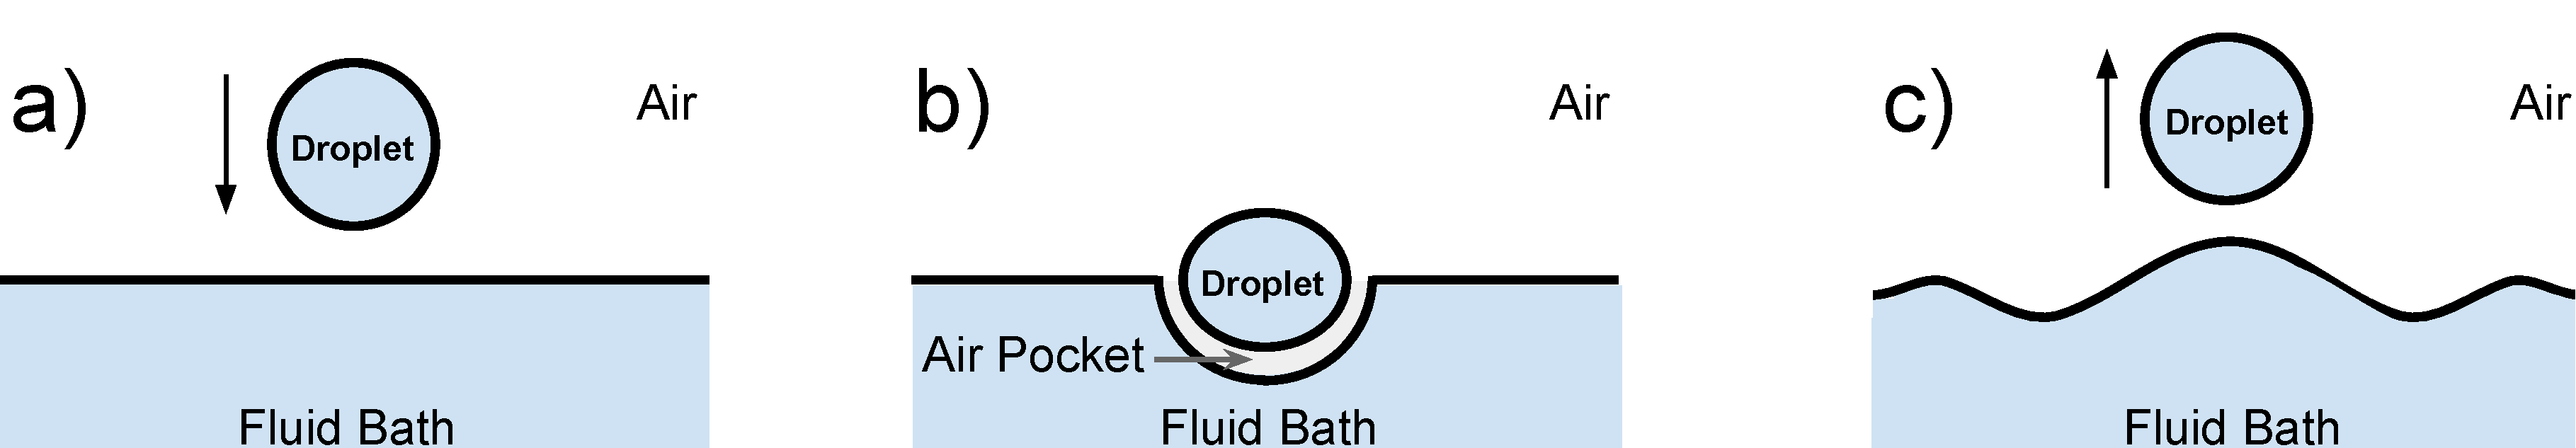
\includegraphics[scale=0.25]{BouncingDroplet.pdf}
	\caption{A depiction of a droplet bouncing on a bath of the same fluid. (a) A droplet falls onto a fluid bath. (b) A film of air gets trapped underneath the droplet. (c) The droplet bounces back up off of the cushion of air.}
	\label{bounce}
\end{figure}
	    
	    Walker found that a trapped film of air kept the droplet and the bath from touching, as shown in \refFig{bounce}. That is, the droplet is bouncing on a layer of air that's struggling to get out of the way but because the bounce happens so quickly, the fluid droplet and the fluid bath never touch. Walker concluded that the leakage rate of this trapped pocket of air depends on three factors: the nature of surface tension of the fluid bath, the viscosity of the droplet and the fluid bath, and the viscocity of the air. The bath must be of uniform surface tension and free from particulate matter floating atop the bath, since both will lead to coalescence. Higher viscosity fluids translate to longer droplet lifetimes, since more viscous fluids keep air from escaping the pocket. Finally, adjusting the frequency and the amplitudes of the vibrations also affects droplet lifetime.\footnote{Reedie Andrew Case ('92) wrote his thesis ``Oil on Troubled Water: The Extension of Floating Drop Lifetimes Due to Interface Vibration" where he looked at droplet lifetime by the frequency of vibration.}   
	     
	    More recent research suggests that a droplet fluid like silicone oil could bounce indefinately of a vibrating bath\rf{Couder2005a}. The long lifetime occurs not only because silicone oil has a high viscosity, but also because it has a \textit{low} surface tension. A low surface tension is beneficial because it makes the oil bath relatively immune to surfactants (surface acting agents) or contaminations which would otherwise make the surface tension nonuniform, and thus create a coalescence event. 

\subsection{Faraday Waves}
	    For a vertically vibrated fluid bath, controlling the amplitude and the frequency of the motion will affect the behaviour of the fluid. Depending on a variety of factors (size of bath, fluid in bath, amplitude, etc.) each system has a specific amplitude (given a specific frequency), which if surpassed, will produce standing surface waves called Faraday waves\rf{Faraday}. \footnote{Faraday waves weren't actually discovered by Michael Faraday, they were originally discovered by X.}~\footnote{Another Reed thesis, this one titled ``Good Vibrations: A Visual Exploration of Faraday Waves" by Alison Saunders, compares mathematical formulation to experimetal results.} A vibrating bath below this critical amplitude, also known as the Faraday instability, will be flat and motionless. A bath with a amplitude greater than the Faraday instability will have a turbulent surface with ripples and waves. An example of Faraday waves is shown in \refFig{faraday waves}. Adjusting the frequency above the Faraday instability will change the size and shape of the Faraday waves. Note that Faraday waves can be created either by increasing amplitude to a critical level, or increasing frequency to a critical level.
	    
	    \begin{figure}[h!]
	\centering
	\includegraphics[scale=0.06]{Faraday.JPG}
	\caption{A picture of Faraday waves in a dish of water at $80~\mathrm{Hz}$.}
	\label{faraday waves}
\end{figure}

\subsection{Walking Droplets}
	    
	A bouncing droplet will bounce differently depending on the frequency and amplitude of the vertical vibrations. If the parameters are set just a hair below the Faraday instability, then a very curious motion arises: the droplet seems to ``walk" accross the surface of the oil. As this \textbf{walker} bounces steadily in a straight line, it encounters a wall and pushes off in another direction, as if from a Newtonian collision. The droplet is being pushed by its own ripples, a dual effort in which niether can exist without the other. In essence, the walker is both a particle and a wave; a conjunction which has only ever been seen at the quantum scale. 
	  
\subsection{Road Map}	  
	  
	Recently, two main groups have been investigating this unique system. A group at MSC in Paris, France, headed by Yves Couder was the first to uncover some of the inherently ``quantum" behaviours of these droplets, in 2005~\cite{Couder2005b}. Since 2010 John Bush's team at MIT have been synthesizing previous experiments, creating a mathematical model, and performing their own investigations of the walker system. A large portion of the literature used in this investigation is drawn from, or at the very least, has its roots in these two groups. 
		
	The thesis documents an experimental investigation into a ``tunneling" behaviour of this bouncing droplet system. While only one other paper really looks at this aspect~\cite{tunneling}, it falls short of completely examining the tunneling behaviour, focusing on barrier width and not examining barrier height. I hope to add the body of work in this subfield by studying how barrier height affects probability of tunneling.   
	
	This thesis is divided into three main chapters. \textbf{Chapter 1} gives a background of the hydrodynamic quantum analogs along with a brief survey of the relevant literature. In \textbf{Chapter 2}, I lay out the experimental design and explain the setup and the data taking procedures. Finally, the results and conclusions are presented in \textbf{Chapter 3}.	    